\chapter*{Discussion}
\label{ch:discussion}
The results presented in the previous chapter show general
uncertainty in the models. This has a few possible explanations:
one of the most likely is the significant overlap of features. This
might explain why all class-wide accuracy plots show the predominance of one
or two classes over the rest. In different trainings, the resulting predominant
classes seem to be chosen at random.\\

There are clear indications of this issue in the recurrent network's performances.
The model presented in the previous chapter shows a general low training accuracy
(figure~\ref{fig:rnn_train_val_acc}), but this was the configuration that
yielded better class-wise accuracies (figures~\ref{fig:rnn_classacc},~\ref{fig:rnn_confmatr}).
With a lower number of epochs, the two predominant classes tendency is worsened, as shown below for an
80 epochs model (figure~\ref{fig:rnn_confmatr80}).
\begin{figure}[H]
    \centering
    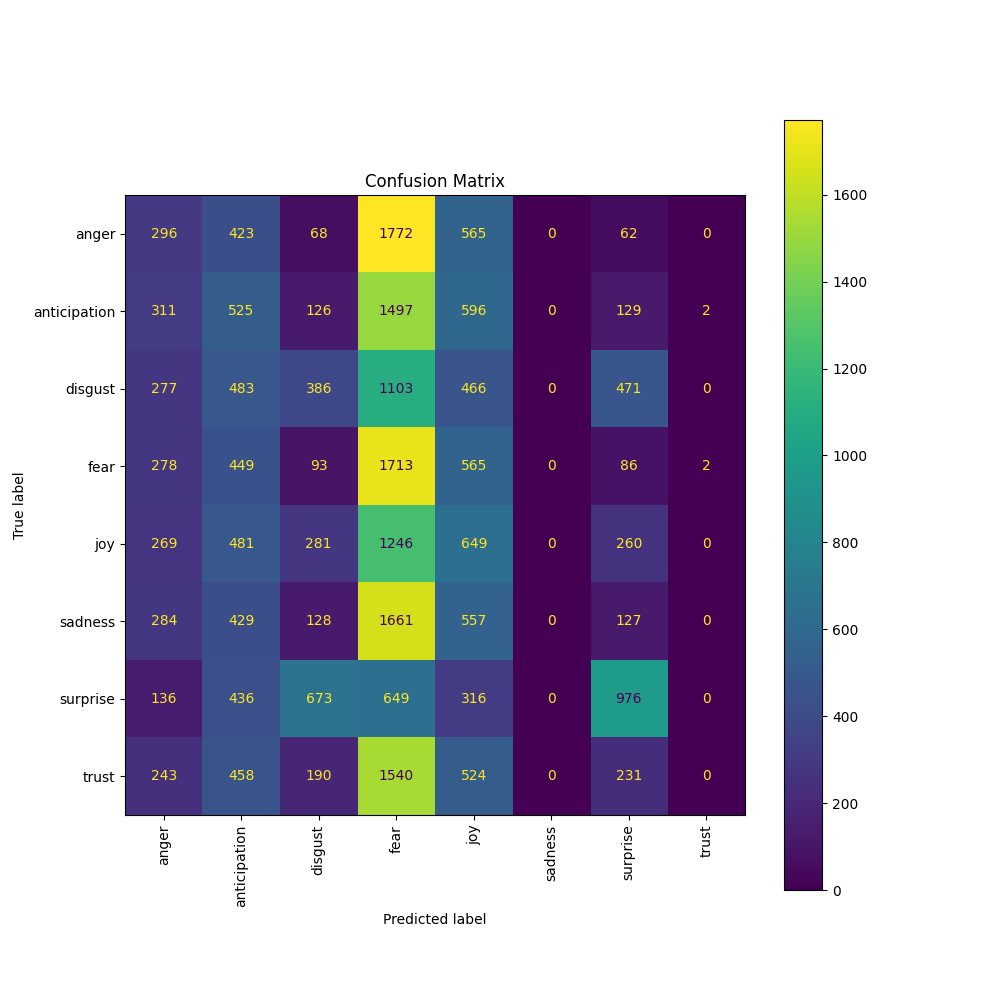
\includegraphics[scale= 0.4]{pictures/rnn_confusion_matrix_80_epochs.png}
    \caption{Confusion matrix for a 80-epochs recurrent neural network}
    \label{fig:rnn_confmatr80}
\end{figure}
It is possible that with higher numbers of epochs the model continues improving
on lower performing classes, but for computational reasons this was not tested.\\
% in the training and validation accuracy plot (figure~\ref{fig:rnn_train_val_acc}):
% once training accuracy begins to rise meaningfully, the model quickly overfits.
% Additional insights are provided by the confusion matrix and class-wise accuracy
% plot (figures~\ref{fig:rnn_confmatr},~\ref{fig:rnn_classacc}), which consistently
% show a dominant class with a high number of predictions and a secondary class
% with relatively high accuracy, while the remaining classes receive significantly
% fewer predictions overall.\\

The convolutional architecture reaches a better training accuracy, but with minimal
corresponding gains in validation accuracy
(figures~\ref{fig:cnn_train_val_acc}).
To a lesser extent, the model also shows the two predominant classes tendency,
as seen in the confusion matrix and class-wise accuracy plot
(figures~\ref{fig:cnn_classacc},~\ref{fig:cnn_confmatr}).\\

Random Forest has better perfomances in this metric as well,
although the issue is still present (as seen in
figures~\ref{fig:cwa_rf},~\ref{fig:roc_rf}).\\

To address this issue, one solution could be applying a filter to exclude the most
common words, allowing the remaining words to better convey clear emotional
meanings. Another potential unexplored approach is the use of custom
metrics during training that focus on class-wise accuracy instead of overall model
accuracy.\\

% \section*{Explainability analysis}
Another probable issue is a flawed ground truth, which may
also contribute to the poor performance and could be linked to the vague distinction
between classes.
This possibility can be investigated through explainability analysis, with an
example provided below (figure~\ref{fig:expl}).

\begin{figure}[H]
    \centering
    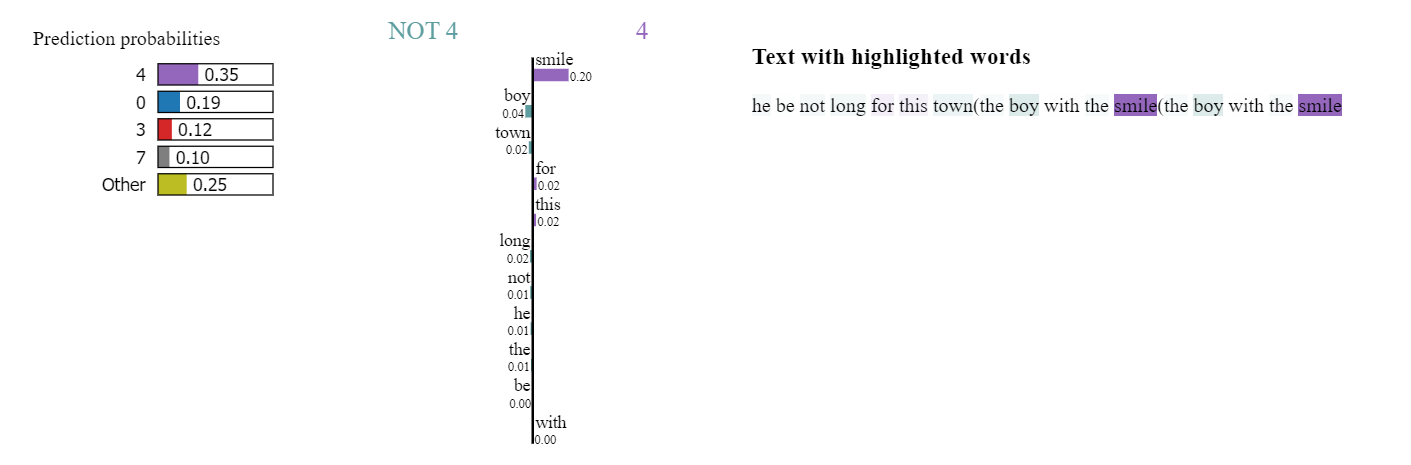
\includegraphics[scale= 0.55]{pictures/expl.png}
    \caption{Explainability - visualization}
    \label{fig:expl}
\end{figure}

The left section of the graph displays the
predicted probabilities for each class. In the center section,
feature importances are ranked from most to least relevant and divided into two
groups: on the right,
features with a positive influence on the predicted label; on the left, those
with a negative influence that suggest the model should consider other classes.
The right section highlights the values of the most important
features, using bright colors to indicate features with a positive influence on the
prediction.
The example in question illustrates a prediction where the model assigned the label \textit{joy} to the stanza under analysis, but the expected label, assigned by the ALBERT model, was \textit{sadness}.
However, the word \textit{smile}, which is brightly highlighted, intuitively suggests that \textit{joy} might be a more plausible class for this stanza, even one that ALBERT could reasonably assign. 
This showcases the aforementioned issue: the transfer learning approach used to
create the ground truth appears to have some limitations. In some instances, labels
generated by ALBERT do not seem to be appropriate.\\

One possible solution is to switch to a different pseudo-labeling model.
Alternatively, using probability vectors rather than direct classification for
labeling could guide the models toward a regression-based approach; this also
allows the ground truth-generator model to provide more context, providing potentially
useful inputs for the models and facilitate a deeper understanding of their
performance issues, helping to identify where and why they struggle.

